\documentclass[tikz,border=8pt]{standalone}
\usepackage[T1]{fontenc}
\IfFileExists{libertine.sty}{\usepackage{libertine}}{}
\IfFileExists{inconsolata.sty}{\usepackage[scaled=0.94]{inconsolata}}{}
\usetikzlibrary{arrows.meta,calc}

\definecolor{navy}{RGB}{35,84,135}
\definecolor{navyfill}{RGB}{241,246,251}
\definecolor{amber}{RGB}{174,106,24}
\definecolor{amberfill}{RGB}{253,248,238}
\definecolor{green}{RGB}{42,116,78}
\definecolor{greenfill}{RGB}{240,248,243}
\definecolor{ink}{RGB}{55,62,69}
\definecolor{muted}{RGB}{104,112,120}

\begin{document}
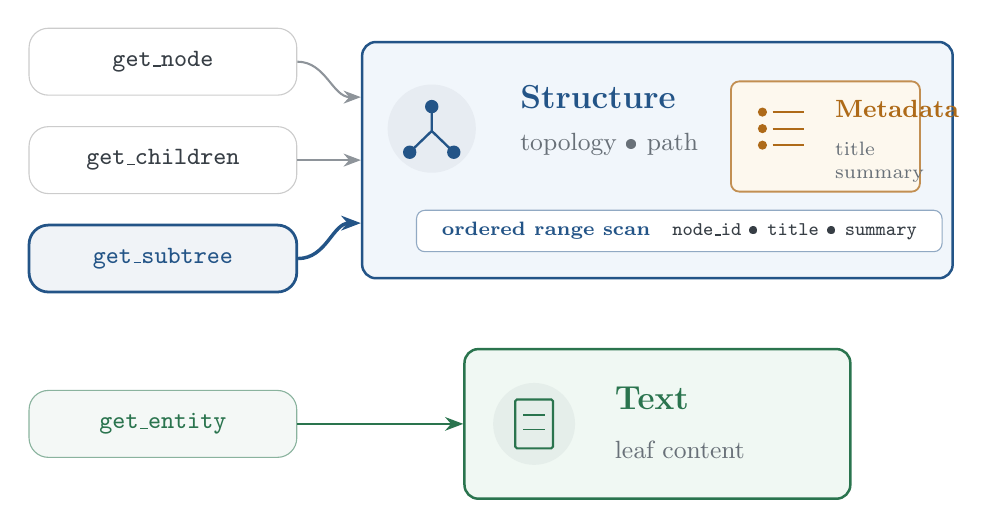
\begin{tikzpicture}[
  api/.style={
    draw=black!20, fill=white, rounded corners=7pt,
    minimum width=34mm, minimum height=8.5mm,
    font=\small\ttfamily, text=ink, align=center
  },
  hotapi/.style={api, draw=navy, fill=navy!7, line width=1pt, text=navy},
  card/.style={
    rounded corners=5pt, line width=0.9pt,
    align=left
  },
  navflow/.style={-{Stealth[length=2.2mm]}, line width=0.75pt, draw=muted!75},
  hotflow/.style={-{Stealth[length=2.5mm]}, line width=1.25pt, draw=navy},
  textflow/.style={-{Stealth[length=2.3mm]}, line width=0.9pt, draw=green}
]

% Storage API rail.
\node[api]    (node)     at (-5.10, 2.45) {get\_node};
\node[api]    (children) at (-5.10, 1.20) {get\_children};
\node[hotapi] (subtree)  at (-5.10,-0.05) {get\_subtree};
\node[api, draw=green!55, fill=green!5, text=green]
              (entity)   at (-5.10,-2.15) {get\_entity};

% Combined structure-and-metadata store.
\node[
  card, draw=navy, fill=navyfill,
  minimum width=75mm, minimum height=30mm
] (combined) at (1.18,1.20) {};

% A slim amber band marks the fields that are co-located with structure.
\fill[amberfill, rounded corners=3pt]
  ([xshift=47mm,yshift=-4mm]combined.west)
  rectangle
  ([xshift=71mm,yshift=10mm]combined.west);
\draw[amber!75, line width=0.65pt, rounded corners=3pt]
  ([xshift=47mm,yshift=-4mm]combined.west)
  rectangle
  ([xshift=71mm,yshift=10mm]combined.west);

% Structure icon: one parent and two children.
\coordinate (sicon) at ([xshift=9mm,yshift=4mm]combined.west);
\fill[navy!11] (sicon) circle (5.6mm);
\draw[navy, line width=0.85pt]
  ($(sicon)+(0,2.7mm)$) -- ($(sicon)+(0,-0.3mm)$)
  ($(sicon)+(0,-0.3mm)$) -- ($(sicon)+(-2.8mm,-3.0mm)$)
  ($(sicon)+(0,-0.3mm)$) -- ($(sicon)+(2.8mm,-3.0mm)$);
\fill[navy] ($(sicon)+(0,2.8mm)$) circle (0.85mm);
\fill[navy] ($(sicon)+(-2.8mm,-3.0mm)$) circle (0.85mm);
\fill[navy] ($(sicon)+(2.8mm,-3.0mm)$) circle (0.85mm);

\node[anchor=west, font=\large\bfseries, text=navy]
  at ([xshift=19mm,yshift=8mm]combined.west) {Structure};
\node[anchor=west, font=\small, text=muted]
  at ([xshift=19mm,yshift=2mm]combined.west) {topology \textbullet\ path};

% Compact metadata-field icon and label.
\coordinate (micon) at ([xshift=52mm,yshift=4mm]combined.west);
\fill[amber] ($(micon)+(-1mm,2.1mm)$) circle (0.58mm);
\fill[amber] ($(micon)+(-1mm,0)$) circle (0.58mm);
\fill[amber] ($(micon)+(-1mm,-2.1mm)$) circle (0.58mm);
\draw[amber, line width=0.7pt]
  ($(micon)+(0.3mm,2.1mm)$) -- ($(micon)+(4.3mm,2.1mm)$)
  ($(micon)+(0.3mm,0)$) -- ($(micon)+(4.3mm,0)$)
  ($(micon)+(0.3mm,-2.1mm)$) -- ($(micon)+(4.3mm,-2.1mm)$);
\node[anchor=west, font=\small\bfseries, text=amber]
  at ([xshift=59mm,yshift=6.5mm]combined.west) {Metadata};
\node[anchor=west, font=\scriptsize, text=muted]
  at ([xshift=59mm,yshift=1.5mm]combined.west) {title};
\node[anchor=west, font=\scriptsize, text=muted]
  at ([xshift=59mm,yshift=-2.0mm]combined.west) {summary};

% The hot subtree operation needs one ordered scan in this layout.
\node[
  anchor=west, rounded corners=3pt,
  draw=navy!50, fill=white, inner xsep=3.2mm, inner ysep=1.5mm,
  font=\scriptsize, text=ink
] at ([xshift=7mm,yshift=-9mm]combined.west)
  {\textcolor{navy}{\bfseries ordered range scan}\quad
   \texttt{node\_id} \textbullet\ \texttt{title} \textbullet\ \texttt{summary}};

% Independent text store.
\node[
  card, draw=green, fill=greenfill,
  minimum width=49mm, minimum height=19mm
] (text) at (1.18,-2.15) {};

\coordinate (ticon) at ([xshift=9mm]text.west);
\fill[green!12] (ticon) circle (5.2mm);
\draw[green, line width=0.75pt, rounded corners=0.6pt]
  ($(ticon)+(-2.4mm,3.1mm)$) rectangle ($(ticon)+(2.4mm,-3.1mm)$);
\draw[green, line width=0.65pt]
  ($(ticon)+(-1.4mm,1.1mm)$) -- ($(ticon)+(1.4mm,1.1mm)$)
  ($(ticon)+(-1.4mm,-0.7mm)$) -- ($(ticon)+(1.4mm,-0.7mm)$);
\node[anchor=west, font=\large\bfseries, text=green]
  at ([xshift=18mm,yshift=3.3mm]text.west) {Text};
\node[anchor=west, font=\small, text=muted]
  at ([xshift=18mm,yshift=-3.3mm]text.west) {leaf content};

% All navigation operations reach the combined store directly.
\draw[navflow] (node.east) to[out=0,in=180] ([yshift=8mm]combined.west);
\draw[navflow] (children.east) -- (combined.west);
\draw[hotflow] (subtree.east) to[out=0,in=180] ([yshift=-8mm]combined.west);
\draw[textflow] (entity.east) -- (text.west);

\end{tikzpicture}
\end{document}
